\documentclass[11pt]{article}

% Change "review" to "final" to generate the final (sometimes called camera-ready) version.
% Change to "preprint" to generate a non-anonymous version with page numbers.
\usepackage[]{acl}
\usepackage{times}
\usepackage{latexsym}

% For proper rendering and hyphenation of words containing Latin characters (including in bib files)
\usepackage[T1]{fontenc}
% For Vietnamese characters
% \usepackage[T5]{fontenc}
% See https://www.latex-project.org/help/documentation/encguide.pdf for other character sets

% This assumes your files are encoded as UTF8
\usepackage[utf8]{inputenc}
\usepackage{microtype}
\usepackage{inconsolata}
\usepackage{graphicx}

% If the title and author information does not fit in the area allocated, uncomment the following
%
%\setlength\titlebox{<dim>}
%
% and set <dim> to something 5cm or larger.

\title{Group 2 Progress Report:\\Binary Genre Classification of Song Lyrics}


\author{Ashwin Unnithan, Arjun Karthik, Kyle Hagerman, Shao Hu\\
  \texttt{\{unnithaa,kartha4,hagermak,hus44\}@mcmaster.ca} }

%\author{
%  \textbf{First Author\textsuperscript{1}},
%  \textbf{Second Author\textsuperscript{1,2}},
%  \textbf{Third T. Author\textsuperscript{1}},
%  \textbf{Fourth Author\textsuperscript{1}},
%\\
%  \textbf{Fifth Author\textsuperscript{1,2}},
%  \textbf{Sixth Author\textsuperscript{1}},
%  \textbf{Seventh Author\textsuperscript{1}},
%  \textbf{Eighth Author \textsuperscript{1,2,3,4}},
%\\
%  \textbf{Ninth Author\textsuperscript{1}},
%  \textbf{Tenth Author\textsuperscript{1}},
%  \textbf{Eleventh E. Author\textsuperscript{1,2,3,4,5}},
%  \textbf{Twelfth Author\textsuperscript{1}},
%\\
%  \textbf{Thirteenth Author\textsuperscript{3}},
%  \textbf{Fourteenth F. Author\textsuperscript{2,4}},
%  \textbf{Fifteenth Author\textsuperscript{1}},
%  \textbf{Sixteenth Author\textsuperscript{1}},
%\\
%  \textbf{Seventeenth S. Author\textsuperscript{4,5}},
%  \textbf{Eighteenth Author\textsuperscript{3,4}},
%  \textbf{Nineteenth N. Author\textsuperscript{2,5}},
%  \textbf{Twentieth Author\textsuperscript{1}}
%\\
%\\
%  \textsuperscript{1}Affiliation 1,
%  \textsuperscript{2}Affiliation 2,
%  \textsuperscript{3}Affiliation 3,
%  \textsuperscript{4}Affiliation 4,
%  \textsuperscript{5}Affiliation 5
%\\
%  \small{
%    \textbf{Correspondence:} \href{mailto:email@domain}{email@domain}
%  }
%}

\begin{document}
\maketitle
% \begin{abstract}
% \end{abstract}

\section{Introduction}

This project investigates the relationship between the linguistic components of songwriting and musical genres by predicting a song's genre primarily on the basis of its lyrics. Although humans typically classify music using a combination of audio and lyrics, this task isolates the English language to determine how specific lyrical themes and structures correspond to music types purely through textual analysis. The overall problem is formatted as a binary single-label classification problem: determining whether an English song belongs to the Pop or Metal genre. Automatic genre detection via lyrics has practical value for the modern music landscape. It serves as a helpful tool to improve end-user recommendation systems on music platforms. In addition, it provides actionable insights for artists and industry professionals on how their music will be categorized and distributed by online recommendation software based on the contextual meaning of their lyrics.

\section{Related Work}

Here, talk about the related work you encountered for your approach. Cite at least 5 references. Refer to item 1. No one has done exactly your task? Write about the most similar thing you can find. This should be around 0.25-0.5 pages.


\section{Dataset}

You should write about your dataset here, following the guidelines regarding item 2. This section may be 0.5-1 pages. Depending on your specific dataset, you may want to include subsections for the preprocessing, annotation, etc.


\section{Features}

Describe any features you used for your model, or how your data was input to your model. Are you doing feature engineering or feature selection? Are you learning embeddings? Is it all part of one neural network? Refer to item 3. This may range from 0.25 pages to 0.5 pages.


Describe any features you used for your model, or how your data was input to your model. Are you doing feature engineering or feature selection? Are you learning embeddings? Is it all part of one neural network? Refer to item 3. This may range from 0.25 pages to 0.5 pages.


\section{Implementation}

Describe your model and implementation here. Refer to item 4. This may take around a page.

This model uses Hugging Face's \textbf{XLNetForSequenceClassification} architecture initialized with the XLNet-base-cased pre-trained checkpoint and tokenizer, with inputs \textbf{padded and truncated to a maximum length of 128 tokens} to ensure consistent dimensions. During training over \textbf{3 epochs} with a \textbf{per-device batch size of 8} (creating an \textbf{effective batch size of 16} via \textbf{2 gradient accumulation steps}), the model utilizes the \textbf{AdamW optimizer}, a \textbf{learning rate of 2e-5}, a \textbf{weight decay of 0.01}, and \textbf{FP16 mixed-precision} to accelerate computation. The task's objective function relies on the standard \textbf{Cross-Entropy Loss} inherent to Hugging Face sequence classification models, and the \textbf{Trainer} is configured to automatically load the \textbf{best-performing weights based on the validation F1-score} at the end of the run.

The model achieved an \textbf{85.21\% accuracy} and an \textbf{85.21\% macro F1-score}, significantly outperforming a \textbf{simple majority-class baseline} (\textbf{F1 = 0.33, Acc = 0.50}) but performing very similar to the \textbf{TF--IDF Logistic Regression baseline} (\textbf{F1 = 0.85, Acc = 0.85}). This similarity in performance is notable: while \textbf{XLNet uses permutation language modeling} to capture \textbf{deep bidirectional semantic context}, TF--IDF relies strictly on \textbf{surface-level word frequency patterns}. The lack of a significant performance gap suggests that the genres in this specific dataset are highly distinguishable through \textbf{surface-level vocabulary cues}, where TF--IDF excels, rather than requiring \textbf{complex contextual semantic understanding}. Alternatively, \textbf{increasing the sequence length beyond 128 tokens} or conducting further \textbf{hyperparameter tuning} might be necessary for the model to further improve its performance.
This model utilizes the \textbf{DistilBERT}-based classification architecture provided by Hugging Face's \texttt{AutoModelForSequenceClassification}. Most importantly, it utilizes a base pretrained version of the model known as \textbf{DistilBERT-base-uncased}. This transformer model was chosen in favour of the complete base version of BERT due to its \textbf{decreased size, computational complexity, and training cost}. Despite this, the model has been proven to retain a \textbf{strong contextual understanding of textual features} during usage. Specifically, the model uses a \textbf{6-layer encoder architecture} compared to the \textbf{12-layer architecture} of the base BERT model. After model importing, it was configured for the \textbf{binary classification task} (song genre classification, Pop and Metal classes) using \textbf{raw lyric textual features} and utilized a standard label mapping of \texttt{p: 0} and \texttt{m: 1} (for easier mapping during downstream training). Initial preprocessing of features (raw lyric text) only involved \textbf{normalizing whitespace} and \textbf{removing null/empty textual records} to retain the original lexical content of the dataset. Afterward, tokenization was conducted using the pretrained \textbf{DistilBERT tokenizer}, which relies on \textbf{WordPiece subword tokenization} (decomposes words into smaller words). WordPiece subword tokenization decomposes a single word into \textbf{multiple smaller tokens} for better size and efficiency. Before passing into the tokenizer, all textual data sequences were \textbf{truncated to a maximum length of 256 tokens}. A token length of \textbf{256} was chosen to allow for \textbf{training and computational efficiency} without largely undermining the \textbf{contextual analysis of lyrics} within the model.

For model fine-tuning, the parameters involved \textbf{2 epochs}, \textbf{input batch size: 16}, \textbf{learning rate: 0.00002}, \textbf{weight decay: 0.01}, and \textbf{warmup steps: 300}. Moreover, during training, the \textbf{Adam optimizer} along with \textbf{cross-entropy loss} (loss function methodology) was used, followed by validation (using the validation set) at the end of each epoch. During training, the \textbf{best-performing checkpoint} was selected using the \textbf{Macro F1 score}. As a result, the final model achieved an \textbf{Accuracy and Macro F1 score of 86.46\%} (\textbf{Accuracy: 0.8646, Macro-F1: 0.8646}) using the test set. Based on the prior baseline performances (baseline performances in Table 1), the \textbf{DistilBERT model outperforms the majority baseline} and \textbf{slightly improves upon the LR + TF-IDF baseline}. This conveys that even though \textbf{class-based lexical classification of lyrics is already strong} (from the LR-based baseline), the introduction of \textbf{contextual semantic text representations} from the DistilBERT model may provide \textbf{slight performance enhancements}.
Another one of our models that we experimented with remains a \textbf{logistic regression} classifier, but extends the TF--IDF baseline by combining three feature types extracted from each lyric. First, we compute \textbf{word-level TF--IDF} features using unigrams and bigrams, removing English stopwords and pruning extremely rare/common terms (\texttt{min\_df=2}, \texttt{max\_df=0.9}), with sublinear TF scaling to reduce the effect of repetition. Second, we add \textbf{character-level TF--IDF} features using 3--6 character n-grams (\texttt{char\_wb}) to capture stylistic patterns such as orthographic variation and elongated spellings that may be missed by word tokenization. Third, we include a small set of \textbf{numeric lyric-structure features} (e.g., word/line counts, bracket-tag count, punctuation, capitalization, and type--token ratio), standardized and concatenated with the sparse TF--IDF vectors. The resulting combined feature vector is used to train logistic regression with L2 regularization (optimized with \texttt{lbfgs}); we tuned the inverse regularization strength and selected $C=8$.

On the balanced validation set, the \textbf{majority-class baseline} achieved \textbf{Accuracy = 0.50} and \textbf{Macro-F1 = 0.33}, while the \textbf{trained TF--IDF + logistic regression baseline} achieved \textbf{Accuracy = 0.85} and \textbf{Macro-F1 = 0.85}. Our proposed feature-engineered model achieved \textbf{Accuracy = 0.873} and \textbf{Macro-F1 = 0.873}, improving over the majority baseline by \textbf{+0.373} accuracy and \textbf{+0.543} macro-F1, and improving over the trained TF--IDF baseline by approximately \textbf{+0.023} on both metrics.
The ELECTRA model was implemented using the standard AutoModelForSequenceClassification and AutoTokenizer from HuggingFace.
Due to its computational efficiency, we were able to maximize the sequence length to ELECTRA's 512 token limit without surpassing available compute.
This was clearly a helpful setting as it outperformed all baselines and models by other groups, making it an effective improvement by giving the model access to the largest possible context during its fine-tuning.

The loss function and optimizer were kept at the default to isolate architectural benefits of ELECTRA in comparison to other models. 
Thus, cross-entropy loss was used as the objective function, which calculates the difference between the predicted probability and actual truth, heavily penalizing the model for being confidently wrong.
The optimizer was Adam with Weight Decay, which pushes the weights towards zero during training to ensure the model remains generalized and does not overfit.
Finally, because this implementation uses a standard architecture, feature ablations were not applicable to this specific model.


\section{Results and Evaluation}

For our task, we use fixed \textbf{train/validation/test} splits for binary lyric genre classification with labels \texttt{p} (Pop) and \texttt{m} (Metal). The original cleaned dataset exhibited a substantial class imbalance (Pop: 86{,}298; Metal: 19{,}133), so we applied \textbf{random downsampling} of the Pop class to match the Metal class count (19{,}133 each), followed by \textbf{stratified splitting} to preserve the class ratio in every split. The resulting data is split \textbf{80/10/10} into Train, Validation, and Test: Train contains 15{,}306 Pop and 15{,}306 Metal examples; Validation contains 1{,}914 Pop and 1{,}913 Metal examples; and Test contains 1{,}914 Pop and 1{,}913 Metal examples. 

We evaluate models primarily using \textbf{Macro-F1}, computed by averaging the F1 scores of each class equally, and secondarily using \textbf{Accuracy}, which measures overall correctness. Macro-F1 is used as the primary metric because it reflects balanced performance across both genres and accounts for both precision and recall, while Accuracy is included as an intuitive secondary measure. 

What are your results? What did you implement and what did your classmates implement? What are your baselines? Refer to items 5 and 6. This may take around 0.5-1 pages.


\section{Error Analysis}

\subsection{Error Artifacts}
\subsubsection{Confusion Matrix}
\begin{figure}[h]
    \centering
    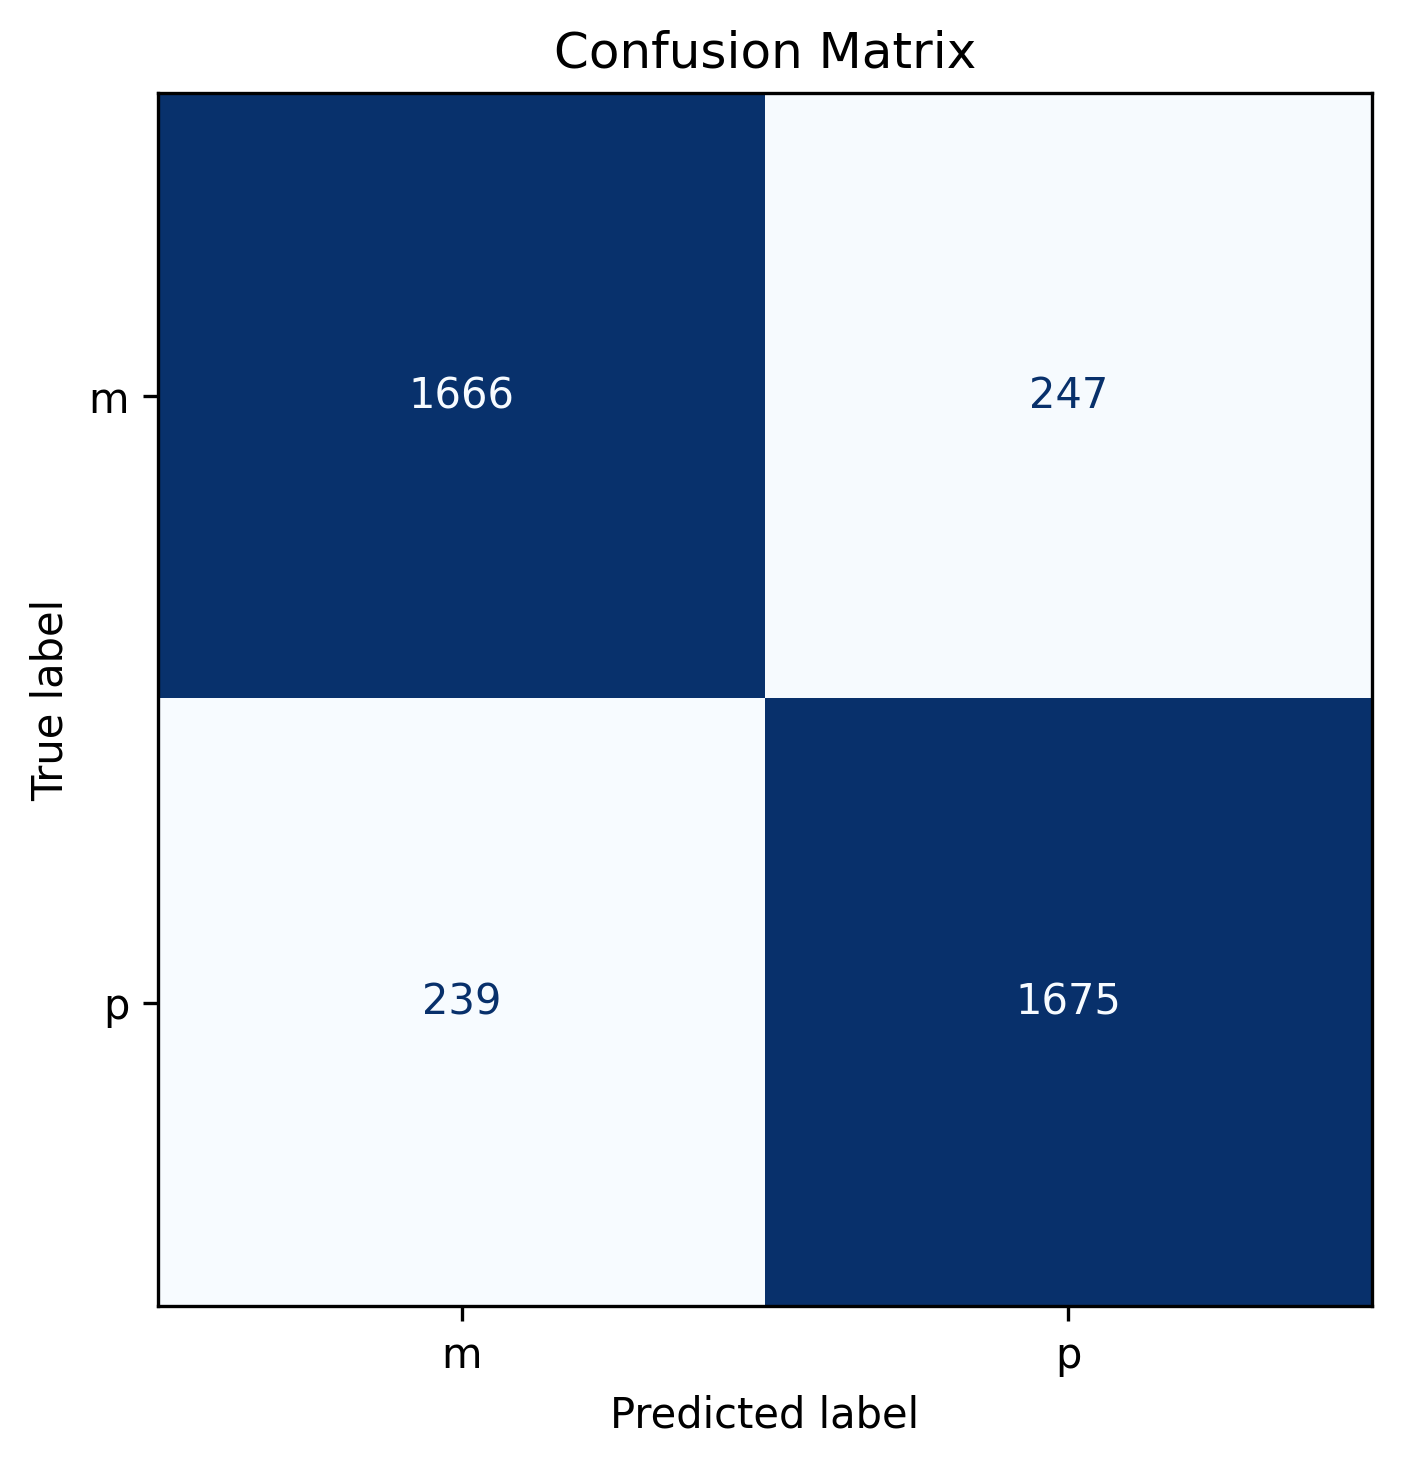
\includegraphics[width=0.4\textwidth]{assets/confusion_matrix_val.png}
    \caption{Confusion Matrix of LR+TF-IDF with Feature Engineering}
    \label{fig:example}
\end{figure}

Based on Figure 1, the confusion matrix shows that the model performs  well across both classes: Pop and Metal. Specifically, 1666 samples of Metal and 1675 samples of Pop were correctly classified. In contrast, only 247 samples of Metal lyrics and 239 samples of Pop were misclassified.

Most importantly, the almost equal error pattern conveys that the model does not exhibit a strong class bias for either genre. This is expected since a strongly balanced dataset distribution was used, as well as the model's intra-class performance (macro F1). The slightly higher correct predictions for Pop indicate marginally better separability for Pop lyrics, though the difference is minimal. Overall, the model appears strong at learning genre-specific lexical and stylistic signals while still encountering difficulty on lyrics with overlapping thematic vocabulary.

\subsubsection{Misclassified Samples}
\begin{table}[h]
\centering
\small
\begin{tabular}{rrrrrr}
\hline
\textbf{Lyric ID} & \textbf{True} & \textbf{Pred} & \textbf{Pred Conf.} & \textbf{Margin} & \textbf{Words} \\
\hline
87199 & m & p & 1.000 & 1.000 & 210 \\
69273 & m & p & 0.999 & 0.999 & 323 \\
5611  & p & m & 0.999 & 0.998 & 110 \\
92588 & m & p & 0.999 & 0.997 & 342 \\
89744 & p & m & 0.999 & 0.997 & 226 \\
82631 & m & p & 0.997 & 0.994 & 197 \\
5246  & m & p & 0.997 & 0.993 & 397 \\
11630 & p & m & 0.996 & 0.992 & 120 \\
7750  & m & p & 0.996 & 0.992 & 407 \\
87716 & m & p & 0.996 & 0.991 & 195 \\
\hline
\end{tabular}
\caption{Top Misclassified Lyric Samples}
\label{tab:misclassified_examples}
\end{table}

As shown in Table 2, the summary of misclassified samples was used to qualitatively analyze the most confident and incorrect model predictions. Specifically, using lyrics (based on lyric IDs) with the highest incorrect prediction confidence, we can identify samples where the model used the wrong features (i.e., lexical cues in the lyrics). Most importantly, after analyzing the textual features (lyrics) of each corresponding lyric ID, a common pattern is shown: the presence of emotional and intense vocabulary that overlaps between both Pop and Metal lyrics. This includes phrases related to pain, love, darkness or conflict. Considering these themes can appear in both genres, it is expected that the likelihood of model confusion with high prediction confidence increases. Moreover, since some songs consist of shorter or highly repetitive lyrics, the lower contextual information may cause additional ambiguity for the model during training and evaluation. As a result, the misclassified sample analysis may suggest that the residual errors of the model are caused by semantic overlap of themes (and related phrases) between the genres rather than issues with the model's parameters or training methodology. 

\subsection{Discussion}
The best performing model was the Logistic Regression model with further feature engineering, compared to the pretrained models tested. When analyzing the model's failures, a thematic challenge emerges regarding context and metaphor. The model was built using a robust feature pipeline that combined word and character n-gram TF-IDF vectors with custom numeric features (like type-token ratio, line counts, and punctuation usage). However, in instances such as song ID 114 and ID 1123, the model incorrectly guessed Pop for Metal songs because the lyrics centered on vulnerability and romance. Lines like "Light me a candle, I'm coming home / Then leave it on your side where I belong" (ID 114) and "Heartbreak and romance / It's better to be numb if you're cracking at the heart" (ID 1123) were misclassified because terms like "home," "heartbreak" and "romance" are statistically dominated by Pop music in the TF-IDF training data, overriding structural features and masking the heavier instrumentation that actually When the model incorrectly guessed Metal for a Pop song, as seen in ID 83472 and ID 60071, the lyrics relied heavily on aggressive metaphors. Lines like "Take away my prime from the mouth of the lion / Savage jaws are the price we pay" (ID 83472) and "Every spark has an ending like a burning fuse" (ID 60071) tricked the model because words like "lion," "savage," "jaws," and "burning" strongly trigger Metal classifications. The primary challenge here is that despite including structural features, the dominant TF-IDF vectors take words literally, failing to recognize when an aggressive word is just a metaphor for a pop breakup or when a soft word is sung over heavy, distorted guitars.

Despite these edge cases, the Logistic Regression pipeline is effective when songs lean into standard genre tropes. For example, a successful Pop classification for song ID 99344 ("head buster off top / grab the chopper and chop / at the top is my spot") demonstrates the model capturing rhythmic, upbeat language and modern slang typical of mainstream hip-hop/pop crossovers. On the other hand, a successful Metal classification for song ID 67457 ("Remnants strewn upon the ground / Drag the carcass withered and brown / Sockets crushed powder remaining") shows the model correctly identifying the overtly dark, morbid, and gothic vocabulary that serves as a staple of the metal genre. In these cases, the semantic meaning perfectly aligns with the literal definitions of the words, allowing the TF-IDF features to confidently and accurately predict the genre based purely on vocabulary frequency.

To improve the robustness of this model and eliminate the literal interpretation blindspots, future iterations should focus on moving beyond strictly frequency-based representations. Additionally, because lyrics only tell half the story, utilizing external APIs to include acoustic features such as energy, tempo, and instrumental features, alongside the existing custom numerical features would immediately resolve ambiguities between songs with similar lyrical themes but vastly different musical styles. 


Overall, the LR+TD-IDF model with feature engineering performs reasonably well with identifying and using correct lexical cues (within lyrics: textual features) for binary genre classification. 

\section{Conclusions}

Summarize your work briefly. Reflect on your implementation and areas for improvement. What do you suggest people work on next (mentioned also in item 7)? This should likely be less than 0.25 pages.


\nocite{mishra2025musicgenreclassificationusing, LI2024e24892, prajuli2026musicgenreclassificationcomparative}


\section*{Team Contributions}

Write in this section a few sentences describing the contributions of each team member. What did each member work on? Refer to item 8.

% Bibliography entries for the entire Anthology, followed by custom entries
%\bibliography{custom,anthology-overleaf-1,anthology-overleaf-2}

% Custom bibliography entries only
\bibliography{custom}

% \appendix

% \section{Example Appendix}
% \label{sec:appendix}

% This is an appendix.

\end{document}
